\chapter{Aplicaciones entre Espacios Topológicos}

\begin{definicion}
    Dados $(X, \cc{T})$, $(Y, \cc{T}')$ dos e.t., diremos que $f : (X, \cc{T}) \to (Y, \cc{T}')$ (que notaremos como $f:X \to Y$ cuando estén claros los e.t.) es \textbf{continua} en un punto $x_0\in X$ si $\forall N'\in \cc{N}_{f(x_0)}'$\ \ $\exists N \in \cc{N}_{x_0}$ con $f(N)\subset N'$. %TODO: dibujo

    \begin{center}
        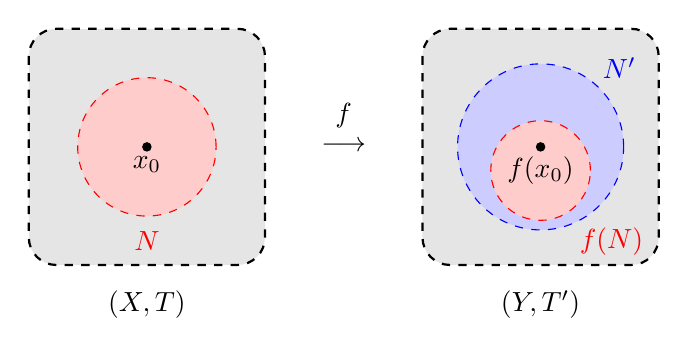
\begin{tikzpicture}
            \def\incolor{gray!20}

            \filldraw[rounded corners=10pt, dashed, thick, fill=\incolor] (0,0) rectangle (3,-3);

            \node at (1.5, -3.5) {$(X, \cc{T})$};
            \node at (4, -1.1) {$f$};
            \node at (4, -1.5) {$\longrightarrow$};

            \filldraw[rounded corners=10pt, dashed, thick, fill=\incolor] (5,0) rectangle (8,-3);

            \node at (6.5, -3.5) {$(Y, \cc{T}')$};

            \filldraw[dashed, draw=red, fill=red!20] (1.5, -1.5) circle (25pt);

            \node at (1.5, -2.7) {\textcolor{red}{$N$}};

            \filldraw[dashed, draw=blue, fill=blue!20] (6.5, -1.5) circle (30pt);

            \filldraw[dashed, draw=red, fill=red!20] (6.5, -1.8) circle (18pt);

            \node at (7.4, -2.7) {\textcolor{red}{$f(N)$}};

            \node at (7.5, -0.5) {\textcolor{blue}{$N'$}};

            \filldraw (1.5, -1.5) circle (1.5pt)  node[below] {$x_0$};

            \filldraw (6.5, -1.5) circle (1.5pt)  node[below] {$f(x_0)$};

            
        \end{tikzpicture}
    \end{center}

    Equivalentemente, $\forall N'\in \cc{N}_{f(x)}'$  $f^{-1}(N')\in \cc{N}_{x_0}$. Es decir, la imagen inversa por f de todo entorno de $f(x)$ en el espacio topológico $\cc{T}'$ es entorno de $x$ en el espacio topológico $\cc{T}$.
    \endsquare
\end{definicion}

\begin{observacion}
    La definición se puede reformular usando abiertos, abiertos básicos o entornos básicos. La demostración queda planteada como ejercicio para el lector. %TODO
    \endsquare
\end{observacion}

\begin{definicion}
    Dados $(X, \cc{T})$, $(Y, \cc{T}')$ dos e.t., $\emptyset \neq A\subset X$. Diremos que $f:X\to Y$ es \textbf{continua en $A$} si es continua en $x$\ \ $\forall x \in A$. Diremos que $f$ es \textbf{continua} si es continua en $X$.
    \endsquare
\end{definicion}

\begin{prop}
    Dados $(X, \cc{T})$, $(Y, \cc{T}')$ dos e.t., $f: X \to Y$. Entonces son equivalentes:
    \begin{enumerate}
        \item[(i)] $f$ es continua.
        \item[(ii)] $f^{-1}(U')\in \cc{T}$\ \ $\forall U' \in \cc{T}$ ($f$ trae abiertos en abiertos).
        \item[(iii)] $f^{-1}(B')\in \cc{T}$\ \ $\forall B'\in \cc{B}'$, donde $\cc{B}'$ es base de $\cc{T}'$.
        \item[(iv)] $f^{-1}(C')\in \cc{C}_{\cc{T}}$\ \ $\forall C' \in \cc{C}_{\cc{T}'}$ ($f$ trae cerrados en cerrados).
        \item[(v)] $f(\overline{A})\subset \overline{f(A)}$\ \ $\forall A \subset X$.
    \end{enumerate}

    \begin{proof}\
        \begin{enumerate}
            \item[(i)$\Rightarrow$(ii)] Supongamos que $f$ es continua. Tomamos $U' \in \cc{T}'$ y tendremos que verificar que $f^{-1}(U')\in \cc{T}$. Sea $x \in f^{-1}(U')$, entonces tendré que ver que $f^{-1}(U')\in \cc{N}_x$. Sabemos que $f(x)\in U' \subset \cc{N}_{f(x)}$. Como $f$ es continua, entonces $\exists U\in \cc{T} $, $x\in U$, $f(U)\subset U' \Rightarrow x \in U \subset f^{-1}(U')$. Como $U\in \cc{T}$, tenemos que $f^{-1}(U')\in \cc{N}_x$. Como esto sucede para un $x$ arbitrario tendremos que se verifica.
            \item[(ii)$\Rightarrow$(iii)] Esta implicación es trivial ya que todo abierto básico es en particular abierto en la topología.
            \item[(iii)$\Rightarrow$(iv)] Sea $C' \in \cc{C}_{\cc{T}'}$, $C'\subset Y$. Tendré que ver que $f^{-1}(C')\in \cc{C}_{\cc{T}}$, lo cual es equivalente a ver que $X \setminus f^{-1}(C')\in \cc{T}$. Sabemos que $X\setminus f^{-1}(C') = f^{-1}(Y\setminus C')$ y $Y\setminus C'\in \cc{T}$. Como $\cc{B}'$ es base de $\cc{T}'$, tenemos que $Y\setminus C'=\bigcup\limits_{i\in I} B_i'$ con $B_i'\in \cc{B}'$\ \ $\forall i \in I$. Entonces tenemos que $f^{-1}(Y\setminus C') = f^{-1}\left(\bigcup\limits_{i\in I}B_i'\right) = \bigcup\limits_{i\in I}f^{-1}(B_i')\in \cc{T}$ por ser unión de abiertos.
            \item[(iv)$\Rightarrow$(v)] Sea $\emptyset \neq A \subset X$, como $\overline{f(A)}\in \cc{C}_{\cc{T}'}$, por (iv) tenemos que $f^{-1}(\overline{f(A)})\in \cc{C}_{\cc{T}}$. Además, $A \subset f^{-1}(f(A))\subset f^{-1}(\overline{f(A)})\in \cc{C}_{\cc{T}}$. Entonces $\overline{A}\subset f^{-1}(\overline{f(A)})$. Al aplicar $f$ tenemos que $f(\overline{A})\subset f(f^{-1}(\overline{f(A)}))=\overline{f(A)}$.
            \item[(v)$\Rightarrow$(iv)] Sea $C' \in \cc{C}_{\cc{T}'}$ y tendremos que ver que $f^{-1}(C')\in \cc{C}_{\cc{T}}$. Para ello veré que coincide con su adherencia, es decir, que $\overline{f^{-1}(C')} = f^{-1}(C')$. Como la inclusión $\overline{f^{-1}(C')} \supset f^{-1}(C')$ es clara tendré que ver solo la otra incusión. Sea $A=f^{-1}(C')$, por (v) tenemos que $f(\overline{f^{-1}(C')})\subset \overline{f(f^{-1}(C'))} \subset \overline{C'}=C'$. Aplicando $f^{-1}$ tenemos que $f^{-1}(f(\overline{f^{-1}(C')}))\subset f^{-1}(C')$ y como $f^{-1}(f(\overline{f^{-1}(C')})) = \overline{f^{-1}(C')}$ tenemos lo buscado.
            \item[(iv)$\Rightarrow$(i)] Sea $x\in X$ arbitrario. Tendré que ver que $f$ es continua en $x$. Sea $U'\in \cc{T}'$ con $f(x)\in U'$. Tendré que ver que existe un $U\in \cc{T}$ con $x\in U$ y $f(U)\subset U'$. Tomo $Y\setminus(U')\in \cc{C}_{\cc{T}'}$ y por (iv) tenemos que $f^{-1}(Y\setminus U')\in \cc{C}_{\cc{T}}$ y $f^{-1}(Y\setminus U') = X \setminus f^{-1}(U')$ por lo que $x\in f^{-1}(U')\in \cc{T}$. Como $f(f^{-1}(U'))\subset U'$ puedo denotar $U = f^{-1}(U')$ y tenemos de nuevo lo buscado. 
        \end{enumerate}
    \end{proof}
\end{prop}

\begin{observacion}
    Si $f: (X, \cc{T}) \to (Y, \cc{T}')$ es una aplicación continua, entonces 
    \begin{gather*}
        f^{-1}((a,b)), f^{-1}((-\infty, b)), f^{-1}((a, +\infty))\in \cc{T}
    \end{gather*}
    y además 
    \begin{gather*}
        f^{-1}([a,b]), f^{-1}((-\infty, b]), f^{-1}([a, +\infty))\in \cc{C}_{\cc{T}}
    \end{gather*}
    La utilidad de esta observación es poder ver si un conjunto es abierto viendo si existe una aplicación continua que lleve un abierto de la topología en dicho conjunto. Análogamente se puede usar para cerrados.
    \endsquare
\end{observacion}

\begin{ejemplo}\
    \begin{itemize}
        \item $f:(X, d) \to (Y, d')$ continua entre espacios métricos 
        \begin{align*}
            \sii &\forall \veps >0\ \ \exists \delta >0 \text{ tal que si } d(x, x_0)<\delta \text{ entonces } d'(f(x), f(x_0))<\veps \sii\\
            \sii &\forall \veps >0 \ \ \exists \delta >0 \text{ tal que } f(B(x_0, \delta))\subset B'(f(x_0), \veps).
        \end{align*}
    \end{itemize}
\end{ejemplo}

\begin{observacion}\
    \begin{itemize}
        \item Cuanto más abiertos hay en $\cc{T}$ y menos en $\cc{T}'$ más fácil es que $f$ sea continua. Por ejemplo, las aplicaciones  
        \begin{align*}
            f:&(X, \cc{T})\to (Y, \cc{T}_t)\\
            f:&(X, \cc{T}_{disc})\to (Y, \cc{T}')
        \end{align*}
        son continuas.

        \item Si $f:(X, \cc{T})\to (Y, \cc{T}')$ es constante, $f(x)=y_0\in Y$\ \ $\forall x \in X$, Sea $U'\in \cc{T}$, entonces
        \begin{gather*}
            f^{-1}=\left\{
            \begin{array}{ccc}
                X & \text{ si }& y_0\in U'\\
                \emptyset & \text{ si } & y_0\notin U
            \end{array}
            \right.
        \end{gather*}

        \item $Id_X : (X, \cc{T}) \to (X, \cc{T}')$ es continua $\sii \cc{T}' \leq \cc{T}$. Por ejemplo, $Id_{\bb{R}}:(\bb{R}, \cc{T}_u)\to (\bb{R}, \cc{T}_S)$ no es continua pero $Id_{\bb{R}}:(\bb{R}, \cc{T}_S) \to (\bb{R}, \cc{T}_u)$ sí lo es.
        \item Si $f:(X, \cc{T})\to (Y, \cc{T}')$ y $g:(Y, \cc{T}')\to (Z, \cc{T}'')$ son aplicaciones continuas, entonces $g\circ f : (X, \cc{T})\to (Z, \cc{T}'')$ es continua.
        \begin{proof}
            Sea $U''\in \cc{T}''$, $(g\circ f)^{-1}(U'') = f^{-1}(g^{-1}(U''))\in \cc{T}$.
        \end{proof}
        \item $f:(X, \cc{T})\to (Y,\cc{T}')$ continua y $\emptyset\neq a  \subset X$, entonces
        \begin{align*}
            f_{|A}:(A, \cc{T}_A) &\to (Y, \cc{T}') \text{ es continua}\\
            x & \mapsto f(x)
        \end{align*}
        \begin{proof}
            Sea $U'\in \cc{T}'$, $(f_{|A})^{-1}(U') = \{x \in A : f(x)\in U\} = f^{-1}(U') \cap A\in \cc{T}_A$ ya que $f^{-1}(U')\in \cc{T}$.
        \end{proof}
        \item Si $f:(X, \cc{T})\to (Y, \cc{T}')$ continua, $\emptyset \neq A' \subset Y$ con $f(X)\subset A'$, entonces 
        \begin{align*}
            f^{A'}:(X, \cc{T}) &\to (A', \cc{T}_{A'}') \text{ es continua}\\
            x &\mapsto f(x)
        \end{align*}
        \begin{proof}
            Sea $O'\in \cc{T}_{A'}'$, entonces $\exists U'\in \cc{T}'$ con $O'=U'\cap A \Rightarrow (f^{A'})^{-1}(O') = (f^{A'})^{-1}(U'\cap A') = f^{-1}(U')\in \cc{T}$ ya que $f$ es continua y $U'$ es abierto en $\cc{T}'$.
        \end{proof}
    \end{itemize}
\end{observacion}

\begin{lema} (de pegado) Sean $(X, \cc{T})$, $(Y, \cc{T}')$ dos e.t. y sea $\{A_i\}_{i\in I}\subset X$ una familia de subconjuntos no vacío de $X$ y $\{f_i:A_i \to Y\}_{i\in I}$ una familia de aplicaciones tales que 
    \begin{enumerate}
        \item[(i)] $\bigcup\limits_{i\in I} A_i =X$.
        \item[(ii)] $f_i=f_j$ en $A_i\cap A_j$\ \ $\forall i,j\in I$ con $A_i\cap A_j \neq \emptyset$. 
        \item[(iii)] $f_i:(A_i, \cc{T}_{A_i})\to (Y, \cc{T}')$ es continua $\forall i \in I$. 
        \item[(iv)] O bien $A_i\in \cc{T}$\ \ $\forall i \in I$ o bien $A_i \in \cc{C}_{\cc{T}}$\ \ $\forall i \in I$ con $I$ finito. 
    \end{enumerate}
    Entonces la aplicación 
    \begin{align*}
        f:(X, \cc{T})&\to (Y, \cc{T}')\\
        x &\mapsto f_i(x) \text{ si }x\in A_i
    \end{align*}
    está bien definida y es continua.
    \begin{proof}\

        Es claro que la aplicación $f$ está bien definida por las condiciones (i) y (ii). Tendremos que ver su continuidad. Tendremos que distinguir dos casos. Demostraremos uno y el otro será análogo y se deja propuesto como ejercicio para el lector:\\

        Supongamos $I$ es finito y $A_i\in \cc{C}_{\cc{T}}$\ \ $\forall i \in I$. Sea $C'\in \cc{C}_{\cc{T}'}$, tendremos que ver que $f^{-1}(C')\in \cc{C}_{\cc{T}}$. Tenemos que $f^{-1}(C') = X\cap f^{-1}(C')\overset{(i)}{=}\left(\bigcup\limits_{i\in I}A_i\right)\cap f^{-1}(C') = \bigcup\limits_{i\in I}(A_i\cap f^{-1}(C')) = \bigcup\limits_{i\in I}\{x\in A : f_i(x)\in C'\} = \bigcup\limits_{i\in I} f_i^{-1}(C')$. Como $f_i^{-1}(C')\in \cc{C}_{\cc{T}_{A_i}}$ y además $A_i\in \cc{C}_{\cc{T}}\Rightarrow f_i^{-1}(C')\in \cc{C}_{\cc{T}}$, entonces por (iv) tenemos que $\bigcup\limits_{i\in I} f_i^{-1}(C')\in \cc{C}_{\cc{T}}$.\\
    \end{proof}
\end{lema}

\begin{ejemplo}
    Sea $f:\bb{R} \to \bb{R}$ definida por
    \begin{gather*}
        f(x)=\left\{
        \begin{array}{ccc}
            \sen(x)=f_1(x) & \text{ si } & x \in (-\infty, 0] = A_1\\
            x^2(x-1)=f_2(x) & \text{ si } & x \in [0,1] = A_2\\
            -\ln(x) = f_3(x) & \text{ si } & x \in [1, +\infty) = A_3\\
        \end{array}
        \right.
    \end{gather*}
    Entonces $f:(\bb{R}, \cc{T}_u) \to (\bb{R}, \cc{T}_u)$ es continua.
    \endsquare
\end{ejemplo}

\section{Aplicaciones abiertas y cerradas}

\begin{definicion}
    Una aplicación $f:(X, \cc{T})\to (Y, \cc{T}')$ diremos que es
    \begin{itemize}
        \item \textbf{abierta} si lleva abiertos de $\cc{T}$ en abiertos de $\cc{T}'$, es decir, $f(U)\in \cc{T}'$\ \ $\forall U \in \cc{T}$.
        \item \textbf{cerrada} si lleva cerrados de $\cc{T}$ en cerrados de $\cc{T}'$, es decir, $f(C)\in \cc{C}_{\cc{T}'}$\ \ $\forall C f\in \cc{C}_{\cc{T}}$.
    \end{itemize}
    \endsquare
\end{definicion}

\begin{observacion}
    Ser continua, abierta y cerrada son propiedades independientes.
    \endsquare
\end{observacion}

\begin{prop}
    Si $f:(X, \cc{T}) \to (Y,\cc{T})$ es una aplicación, entonces equivalen:
    \begin{enumerate}
        \item[(i)] $f$ es abierta.
        \item[(ii)] $f(B)\in \cc{T}'$\ \ $\forall B \in \cc{B}$ con $\cc{B}$ base de $\cc{T}$.
        \item[(iii)] Si  $x\in X$, $N\in \cc{N}_x$, entonces $f(N)\in \cc{N}_{f(x)}'$.
        \item[(iv)] Si $A\subset X$, entonces $f(A^\circ)\subset (f(A))^\circ$.
    \end{enumerate}
    \begin{proof}\
        \begin{itemize}
            \item[(i)$\Rightarrow$(ii)$\Rightarrow$(iii)] Trivial.
            \item[(iii)$\Rightarrow$(iv)] Sea $x\in A^\circ$, tendremos que ver que $f(x)\in (f(A))^\circ$. Como $x\in A^\circ$, entonces $A\in \cc{N}_x$ y por (iii) tenemos que $f(A)\in \cc{N}_{f(x)}'$ por lo que $f(x)\in (f(A))^\circ$.
            \item[(iv)$\Rightarrow$(i)] $U\in \cc{T}$ por lo que $U=U^\circ$. Entonces $f(U) = f(U^\circ)$ y por (iv) tenemos que $f(U^\circ)\subset (f(U))^\circ$  y como la otra inclusión se da siempre tenemos que $f(U)=(f(U))^\circ\in \cc{T}$.
        \end{itemize}
    \end{proof}
\end{prop}

\begin{prop}
    Si $f:(X, \cc{T}) \to (Y,\cc{T})$ es una aplicación, entonces equivalen:
    \begin{enumerate}
        \item[(i)] $f$ es cerrada.
        \item[(ii)] $\overline{f(A)}\subset f(\overline{A})$\ \ $\forall A \subset X$.
    \end{enumerate}
    \begin{proof}\
        \begin{itemize}
            \item[(i)$\Rightarrow$(ii)] $\overline{A}\in \cc{C}_{\cc{T}} \overset{(i)}{\Rightarrow} f(\overline{A}\in \cc{C}_{\cc{T}})$ y como  $\overline{f(A)} \subset f(\overline{A})$ lo tenemos.
            \item[(ii)$\Rightarrow$(i)] $\overline{C}=C\in \cc{C}_{\cc{T}}$, por (ii) tenemos que $\overline{f(C)}\subset f(\overline{C})= f(C) \in \cc{C}_{\cc{T}'}$. 
        \end{itemize}
    \end{proof}
\end{prop}